\documentclass[a4paper,12pt]{report}
% safe参数解决与\!在内的多个冲突
% \sups命令可能被重定义,xeCJK放在tipa后
\usepackage[safe]{tipa}

% 中文支持
\usepackage[slantfont,boldfont]{xeCJK}
	\setCJKmainfont[BoldFont=SimHei,ItalicFont=KaiTi]{SimSun}
	\setCJKmathfont{STXinwei}
\usepackage{indentfirst}

% 数学环境
\usepackage{amsmath}
  \newcommand{\ue}{\mathrm{e}}
  \newcommand{\ud}{\mathop{}\negthinspace\mathrm{d}}
\usepackage{amssymb}
\usepackage{mathrsfs} % 线性代数字体
    % overline的替代命令
\newcommand{\closure}[2][3]{{}\mkern#1mu\overline{\mkern-#1mu#2}}
\usepackage{yhmath} % 左下-右上省略号
\usepackage{mathtools} % dcases环境
\usepackage{amsthm} % 定理环境
  \theoremstyle{definition}\newtheorem{laws}{Law}[section]
  \theoremstyle{plain}\newtheorem{ju}[laws]{Jury}
  \theoremstyle{remark}\newtheorem*{marg}{Margaret}
\usepackage{esint} % 多重积分,需放在amsmath后

% 下划线宏包
\usepackage{ulem}
% LaTeX符号宏包
\usepackage{hologo}
	\newcommand{\xelatex}{\Hologo{XeLaTeX}}
	\newcommand{\bibtex}{\Hologo{BibTeX}}
% 其他符号
\usepackage{wasysym}
% 带箱小页
\usepackage{boxedminipage}
% 绘图
\usepackage{tikz}
	\usetikzlibrary{calc}
	\newcommand{\tikzline}[1]{{#1\tikz{\draw[#1,line width=9](0,0)--(0.5,0);}}, }

% 奇怪的小定义
\newcommand{\dpar}{\\ \mbox{}}	% 空两行
\newcommand{\qd}[1]{{\bfseries{#1}}}	% 强调
\newcommand{\co}[1]{{\bfseries{#1}}}   % Style of concept
\newcommand{\RED}[1]{{\color{red}{#1}}}
\newcommand{\cmmd}[1]{\fbox{\texttt{\char92{}#1}}}
\newcommand{\charef}[1]{第\ref{#1}章}
\newcommand{\secref}[1]{第\ref{#1}节}
\newcommand{\pref}[1]{第\pageref{#1}页}
\newcommand{\fref}[1]{图\ref{#1}}
\newcommand{\tref}[1]{表\ref{#1}}

% 编号列表宏包,并自定义了三个列表
%\usepackage[inline]{enumitem}
%	\setlist[enumerate]{label=\arabic* - ,font=\bfseries,itemsep=0pt}
%	\setlist[itemize]{label=$\bullet$,font=\bfseries,leftmargin=\parindent}
%	\setlist[description]{font=\bfseries\uline}
%
%\newenvironment{fead}{\setlength{\parskip}{0pt}
%	\begin{description}[font=\bfseries\uline,labelindent=\parindent]
%		\setlength{\itemsep}{0pt}\setlength{\parsep}{0pt}\setlength{\parskip}{0pt}}
%	{\end{description}}
% 带宽度的
\newenvironment{para}{\setlength{\parskip}{0pt}
	\begin{description}[font=\bfseries\ttfamily]
		\setlength{\itemsep}{0pt}\setlength{\parsep}{0pt}\setlength{\parskip}{0pt}}
	{\end{description}}
\newenvironment{feae}{\setlength{\parskip}{0pt}
	\begin{enumerate}[font=\bfseries,labelindent=0pt]}
	{\end{enumerate}}
\newenvironment{feai}{\setlength{\parskip}{0pt}
	\begin{itemize}[font=\bfseries]
		\setlength{\itemsep}{0pt}\setlength{\parsep}{0pt}\setlength{\parskip}{0pt}}
	{\end{itemize}}
\newenvironment{inlinee}
{\begin{enumerate*}[label=(\arabic*), font=\rmfamily, before=\unskip{:},itemjoin={{;}},itemjoin*={{,以及:}}]}
	{\end{enumerate*}。}

% 目录和章节样式
\usepackage{titlesec}
\usepackage{titletoc}   % 用于目录

\titlecontents{chapter}[1.5em]{}
	{\contentslabel{1.5em}}{\hspace*{-2em}}{\hfill\contentspage}
	
\titlecontents{section}[3.3em]{}
	{\contentslabel{1.8em}}
	{\hspace*{-2.3em}}
	{\titlerule*[8pt]{$\cdot$}\contentspage}
%	
\titlecontents{subsection}[2.5em]{\small}
	{\thecontentslabel{} }
	{}
	{\titlerule*[5pt]{$\cdot$}\contentspage}
 %章节样式
\setcounter{secnumdepth}{3} % 一直到subsubsection
\newcommand{\chaformat}[1]{%
	\parbox[b]{.5\textwidth}{\hfill\bfseries #1}%
	\quad\rule[-12pt]{2pt}{70pt}\quad
	{\fontsize{60}{60}\selectfont\thechapter}}
\titleformat{\chapter}[block]{\hfill\LARGE\sffamily}{}{0pt}{\chaformat}[\vspace{2.5pc}\large
	\startcontents\printcontents{}{1}{\setcounter{tocdepth}{2}}]
%\titleclass{\section}{top}
%\titleformat{\section}{\Large\bfseries}{\thesection}{0.5em}{}
\titleformat*{\section}{\centering\Large\bfseries}
\titleformat{\subsubsection}[hang]{\bfseries\large}{\rule{1.5ex}{1.5ex}}{0.5em}{}
% 扩展章节
\newcommand{\starsec}{\noindent\fbox{\S\textit{注意:本章节是一个扩展阅读章节。}}
	\\ \mbox{}}

\renewcommand{\contentsname}{目录}
	\renewcommand{\tablename}{表}
	\renewcommand\arraystretch{1.2}	% 表格行距
	\renewcommand{\figurename}{图}
% 设置不需要浮动体的表格和图像标题
\setlength{\abovecaptionskip}{5pt}
\setlength{\belowcaptionskip}{3pt}
\makeatletter
\newcommand\figcaption{\def\@captype{figure}\caption}
\newcommand\tabcaption{\def\@captype{table}\caption}
\makeatother
% 图表
\usepackage{array,multirow}
  \setlength\extrarowheight{2pt} % 行高增加
\usepackage{longtable}
\usepackage{graphicx}
  \graphicspath{{./tikz/}}
% 页面修正宏包
\usepackage[top=1in]{geometry}

% 代码环境
\usepackage{listings}
% Avoid copy line numbers of the listing code (Invalid for SumatraPDF Reader)
\usepackage{accsupp}
	\newcommand{\emptyaccsupp}[1]{\BeginAccSupp{ActualText={}}#1\EndAccSupp{}}
% Color
\usepackage{xcolor}
	\definecolor{commentcolor}{RGB}{85,139,78}
	\definecolor{numbercolor}{RGB}{166,206,168}
	\definecolor{stringcolor}{RGB}{206,145,108}
	\definecolor{keywordcolor}{RGB}{34,34,250}
	\definecolor{backcolor}{RGB}{220,220,220}
	\definecolor{packagecolor}{RGB}{0,128,0}
	\definecolor{envicolor}{RGB}{185,70,15}
% LaTeX Code Style
%\lstset{language=[LaTeX]TeX,
%		basicstyle=\small\ttfamily,
%		commentstyle=\color{commentcolor},
%		keywordstyle=\color{keywordcolor},
%		stringstyle=\color{stringcolor},
%		showstringspaces=false,
%		% Package/Tikz-Lib Using
%		classoffset=0,
%		morekeywords={begin,end,usetikzlibrary},
%		keywordstyle=\color{keywordcolor},
%		classoffset=1,
%		morekeywords={article,report,book,
%			xeCJK,tikz,
%			calc},
%		keywordstyle=\color{packagecolor},
%		classoffset=2,
%		morekeywords={document,tikzpicture},
%		keywordstyle=\color{envicolor},
%		% Line Number Style
%		numbers=left,
%		numberstyle=\tiny\emptyaccsupp,
%		stepnumber=1,
%		% Frame and Background Color
%		frame=single,
%		framerule=0pt,
%		backgroundcolor=\color{backcolor},
%		% Spaces
%		% belowskip=\medskipamount,
%		emptylines=1,
%		escapeinside=``}

\lstnewenvironment{latex}[1]{\lstset{#1}}{}
\newcommand{\latexline}[1]{{\lstinline[language=TeX,basicstyle=\small\ttfamily]{#1}}}

% Tikz Code
\lstdefinelanguage{tikzlang}{
	classoffset=0, % 蓝色的keyword
	morekeywords={begin,end,newcommand,
		draw,node,coordinate,tikzstyle,foreach},
	keywordstyle=\color{keywordcolor},
	classoffset=1, % 棕色的其他关键字
	morekeywords={tikzpicture,grid,at,
		thick,thin,very,ultra,
		red,green,yellow,blue,cyan,magenta,black,
		    gray,darkgray,lightgray,brown,lime,
		    olive,orange,pink,purple,teal,violet,white},
	keywordstyle=\color{envicolor},
	morecomment=[l]{\%},
	morecomment=[s]{/*}{*/},
	morestring=[b]',
	% Escape
	escapeinside=``
}
\lstnewenvironment{tikzcode}[1]{\lstset{language=tikzlang,basicstyle=\small\ttfamily,
		breaklines=true,%backgroundcolor=\color{white},
		linewidth=0.7\linewidth,#1}}{}

% 附录
\usepackage{appendix}

% 行号
\usepackage{lineno}

% 代码输入环境
%\usepackage{verbatim,xcolor}
%\newbox\savedlines
%\newtoks\savedtokens
%\makeatletter
%\def\codeshow{%
%\global\savedtokens={}%
%\def\verbatim@processline{%
%{\setbox0=\hbox{\the\verbatim@line}%
%\hsize=\wd0
%\the\verbatim@line\par}%
%\global\savedtokens=\expandafter{\the\expandafter\savedtokens\the\verbatim@line^^J}}%
%\@tempswatrue
%\setbox0=\vbox\bgroup\parskip=0pt\topsep=0pt\partopsep=0pt
%\verbatim}
%\def\endcodeshow{\endverbatim%
%\unskip\setbox0=\lastbox\egroup
%\global\setbox\savedlines=\box0
%\addvspace{1em}\par\noindent%
%\colorbox{lightgray}{%
%\begin{minipage}{.55\textwidth}{\usebox\savedlines}\end{minipage}}%
%\hfill\fbox{\parbox{.40\textwidth}%
%{\scantokens\expandafter{\the\savedtokens\unskip\endinput}}}%
%\par\addvspace{1em}}
%\makeatother

% 引用
\usepackage[colorlinks,bookmarksopen=true,bookmarksnumbered=true]{hyperref}

%\documentclass{ctexart}
\usepackage{listings}
\usepackage{algorithm}
\usepackage{amsmath,bm}
\usepackage{algorithmic}
\lstset{
linewidth=1.1\textwidth,
numbers=left, 
numberstyle= \footnotesize, 
keywordstyle= \color{ blue!70},
commentstyle=\color{red!50!green!50!blue!50}, 
frame=shadowbox, 
backgroundcolor=\color[RGB]{245,245,244},
%escapeinside=``, %逃逸字符(1左面的键),用于显示中文
breaklines,
extendedchars=false, %解决代码跨页时,章节标题,页眉等汉字不显示的问题
xleftmargin=2em,xrightmargin=2em, aboveskip=1em, %设置边距
tabsize=4, %设置tab空格数  
showspaces=false %不显示空格 
rulesepcolor= \color{ red!20!green!20!blue!20} 
}
\title{数值分析第一次大作业}
\author{张晋\\学号:15091060}
\date{最后更新于:\today}
\begin{document}

\maketitle

\tableofcontents


\newpage

\chapter{题目}
设有$501\times501$的实对称矩阵$\bm{A}$,
\[\bm{A}=\left[ {\begin{array}{*{20}{c}}
a_1&b&c&{}&{}\\
b& \ddots& \ddots& \ddots &{}\\
c& \ddots& \ddots& \ddots &c\\
{}& \ddots& \ddots& \ddots &b\\
{}&{}& c& b&{a_{501}}
\end{array}} \right]\]
其中:

$a_i=(1.64-0.024i)sin(0.2i)-0.64e^{\frac{0.1}{i}}
(i=1,2,\cdots,501)$

$b=0.16$

$c=-0.064$

矩阵$\bm{A}$的特征值为$\lambda_i(i=1,2,\cdots,501)$
并且有
\[{\lambda _1} \le {\lambda _2} \le {\lambda _3} \le  \cdots  \le {\lambda _{501}},\left| {{\lambda _s}} \right| = \mathop {\min }\limits_{1 \le i \le 501} \left| {{\lambda _i}} \right|\]

\begin{enumerate}
\item 求$\lambda _1,\lambda _{501}$和$\lambda_s$的值。
\item 求$\bm{A}$的与数${\mu _{k}} = {\lambda _1} + k\dfrac{{{\lambda _{501}} - {\lambda _1}}}{{40}}$最接近的特征值
${\lambda _{{i_k}}}(k=1,2,\cdots,39)$。
\item 求$\bm{A}$的(谱范数)条件数$cond(\bm{A})_2$和行列式
$det\bm{A}$

\end{enumerate}
\newpage
\chapter{算法设计方案}
\section{基本算法}
\subsection{幂法}
幂法是一种求实矩阵$A$的按模最大的特征值$\lambda_1$及其对
应的特征向量$\bm{x}_1$的方法。特别适合于大型稀疏矩阵。

设${\bm{A}} = {({a_{ij}})_{n \times n}} \in {\mathbb{R}^{n \times n}}$有一个完全特征向量组, 其特征值为${\lambda _1},{\lambda _2}, \cdots ,{\lambda _n}$,对应的特征向量为${\bm{x}_1},{{\bm{x}}_2}, \cdots ,{{\bm{x}}_n}$。

并设A的主特征值是实根,且满足
\[{\rm{  }}\left| {{\lambda _1}} \right| > \left| {{\lambda _2}} \right| \ge  \cdots  \ge \left| {{\lambda _n}} \right|\]
现在讨论求$\lambda _1$及$\bm{x}_1$的基本方法.
\begin{align*}
\forall {{\bm{v}}_0} &= {a_1}{{\bm{x}}_1} + {a_2}{{\bm{x}}_2} +  \cdots  + {a_n}{{\bm{x}}_n},
(设{a_1} \ne 0)\\
{{\bm{v}}_1} &= {\bm{A}}{{\bm{v}}_0} = {a_1}{\lambda _1}{{\bm{x}}_1} + {a_2}{\lambda _2}{{\bm{x}}_2} +  \cdots  + {a_n}{\lambda _n}{{\bm{x}}_n}\\
\cdots\\
{{\bm{v}}_k} &= {\bm{A}}{{\bm{v}}_{k - 1}} = \lambda _1^k\left[ {{a_1}{{\bm{x}}_1} + {a_2}{{\left( {\frac{{{\lambda _2}}}{{{\lambda _1}}}} \right)}^k}{{\bm{x}}_2} +  \cdots  + {a_n}{{\left( {\frac{{{\lambda _n}}}{{{\lambda _1}}}} \right)}^k}{\bm{x}_n}} \right]
\end{align*}

当$k$很大时,有
\[{{\bm{v}}_k} \approx \lambda _1^k{a_1}{{\bm{x}}_1}\]
\[{{\bm{v}}_{k + 1}} \approx {\lambda _1}{{\bm{v}}_k}\]
\[{\bm{A}}{{\bm{v}}_k} \approx {\lambda _1}{{\bm{v}}_k}\]
\[\mathop {{\rm{lim}}}\limits_{k \to \infty } \dfrac{{{{\bm{v}}_k}}}{{\lambda _1^k}} = {a_1}{{\bm{x}}_1}
\]

即$\bm{v}_k$是$\lambda_1$的近似的特征向量.
而主特征值
\[{\lambda _1} \approx \dfrac{{{{({{\bm{v}}_{k + 1}})}_j}}}{{{{({{\bm{v}}_k})}_j}}}\]

那么若我们要求某个$n$阶方阵$A$的特征值和特征向量,
可以先任取一个初始向量$\bm{x}_0$,
构造序列$\{\bm{x}_{k=1}^{\infty}\}$,
其中$\bm{x}_k:=\bm{A}\bm{x}_{k-1}$
那么当$k$充分大时,$\bm{x}_k$可近似作为矩阵$\bm{A}$的特征值。

实际运算时为避免$\bm{x}_k$的模过大或过小,
通常每迭代一次都对$\bm{x}_k$进行归一化。

算法过程如下:

(1) 任取一个长度为$n$的非零列向量$\bm{x}_i$;

(2) 用矩阵$\bm{A}$乘以$\bm{x}_i$,
得到列向量$\bm{x}_{i+1}=\bm{A}\bm{x}_i$;

(3) 标准化列向量$\bm{x}_{i+1}$,也就是表示成一个因子 (绝对值最大的元素的倒数) 乘以$\bm{x}_{i+1}$,使得$\bm{x}_{i+1}$中最大的元素是$1$;

(4) 将$\bm{x}_{i+1}$(不包括上面的因子) 作为 (1) 中的$\bm{x}_i$重复 (1) 中的操作。
这个迭代过程一直进行,直到相邻两个列向量$\bm{x}_{i}$和$\bm{x}_{i+1}$的差异满足一定的条件,这个差异可以用多种方式进行衡量,
如果使用无限范数来衡量即是
\[{\Vert \bm{x}_{i+1}-\bm{x}_i\Vert}_\infty \le tol\]

大的特征值就是当前$\bm{x_{i+1}}$进行标准化得到的因子。幂法肯定是会收敛的,如果初始列向量和特征向量很接近的话收敛会很快,否则会很慢。
\textit{幂法只能算出最大的特征值,
并且最大的特征值不能是特征方程的重根,
其次,最大特征值必须是实数}。

程序伪代码如下:
\begin{algorithm}
  \caption{The Power Method}
  \label{alg1}
  \begin{algorithmic}[1]
 	\STATE Choose a random vector $\bm{u}_{0}\in \mathbb{R}^{n}$
  \WHILE{$|\beta_{k}-\beta_{k-1}|>\epsilon$}
  \STATE $\bm{y}_{k-1}=\bm{u}_{k-1}/\Vert \bm{u}_{k-1}\Vert$
  \STATE $\bm{u}_{k}=\bm{A}\bm{y}_{k-1}$
  \STATE $\beta_{k}=\bm{y}_{k-1}^{T}\bm{u}_{k}$
  \ENDWHILE
  \end{algorithmic}
\end{algorithm}

\newpage
\subsection{反幂法}
反幂法可求非奇异实矩阵的按模最小特征值及特征向量
由于矩阵$A$的特征值$\lambda$的倒数就是矩阵
$A^{-1}$的特征值,
所以,如果对$A^{-1}$
进行同样的幂法过程,那么就可以得到矩阵$A$的最小的特征值,这种方法就叫
做反幂法。

程序伪代码如下:
\begin{algorithm}
  \caption{The Inverse Power Method}
  \label{alg2}
  \begin{algorithmic}[1]
 	\STATE Choose a random vector $\bm{u}_{0}\in \mathbb{R}^{n}$
  \WHILE{$|\beta_{k}-\beta_{k-1}|>\epsilon$}
  \STATE $\bm{y}_{k-1}=\bm{u}_{k-1}/\Vert \bm{u}_{k-1}\Vert$
  \STATE $\bm{u}_{k}=\bm{A}^-1\bm{y}_{k-1}$
  \STATE $\beta_{k}=\bm{y}_{k-1}^{T}\bm{u}_{k}$
  \ENDWHILE
  \end{algorithmic}
\end{algorithm}

PS:其中$\bm{u}_k$通常由$Doolittle$分解法求得

\subsection{移位幂法}
如果得到了矩阵$A$的最大或者最小的特征值,那么使用移位幂法可以
得到其他的特征值。它的原理是:假设$ax =\lambda_1x$,
其中$\lambda_1$是通过幂法求得的矩阵的最大的特征值,
那么新的移位矩阵[$a−\lambda_1*I$]的特征值便是
$\lambda_2-\lambda_1, \lambda_3-\lambda_1,
\cdots,\lambda_n-\lambda_1$。
移位矩阵的特征向量和原矩阵的特征向量是一样的。
如果对移位矩阵也应用基本幂法,得到特征值$\alpha_k$,
那么原矩阵的特征值$\lambda_k= \alpha_k+\lambda_1$。不断重复上面的过程$k-2$次,便可以得到原矩阵的所有的特征值

\subsection{Doolittle分解法}
\textbf{定义:}杜尔里特算法(Doolittle algorith)从下至上地对矩阵A做初等行变换,将对角线左下方的元素变成零,然后再证明这些行变换的效果等同于左乘一系列单位下三角矩阵,这一系列单位下三角矩阵的乘积的逆就是L矩阵,它也是一个单位下三角矩阵。本质上是高斯消元法的一种表达形式。

\textbf{复杂度:}时间复杂度一般在$\frac{2n^{3}}{3}$左右。空间复杂度为$n^2$,只占用一个储存矩阵$\bm{A}$的数组。

具体步骤如下:

对给定的$N\times N$矩阵
${\displaystyle A=(a_{n,n})}$

有
${\displaystyle A^{(0)}:=A} $

然后定义对于$n = 1,\cdots,N-1$的情况如下:

在第$n$步,消去矩阵$A^{(n-1)}$的第$n$列主对角线下的元素:

将$A^{(n-1)}$的第$n$行乘以
\[{\displaystyle l_{i,n}:=-{\frac {a_{i,n}^{(n-1)}}{a_{n,n}^{(n-1)}}}}\]

之后加到第$i$行上去。
其中${\displaystyle i=n+1,\cdots ,N}$ 

这相当于在$\bm{A}^{(n-1)}$的左边乘上一个单位下三角矩阵:
\[L_{n}={\begin{pmatrix}1&&&&&0\\&\ddots &&&&\\&&1&&&\\&&l_{{n+1,n}}&\ddots &&\\&&\vdots &&\ddots &\\0&&l_{{N,n}}&&&1\\\end{pmatrix}}\]

于是设:
\[{\displaystyle A^{(n)}:=L_{n}A^{(n-1)}}\]
经过$N-1$轮操作后,所有在主对角线下的系数都为$0$了,
于是我们得到了一个上三角矩阵:$A^{(n-1)}$,这时就有:

\begin{align*}
A&= L_1^{ - 1}{L_1}{A^{(0)}}\\
 &= L_1^{ - 1}{A^{(1)}}\\
 &= L_1^{ - 1}L_2^{ - 1}{L_2}{A^{(1)}}\\
 &= L_1^{ - 1}L_2^{ - 1}{A^{(2)}}\\
 &=  \ldots \\
 &= L_1^{ - 1} \ldots L_{N - 1}^{ - 1}{A^{(N - 1)}}
\end{align*}

这时,矩阵$A^{(n-1)}$就是$U$,
\[\displaystyle L=L_{1}^{-1}\ldots L_{N-1}^{-1}\]
下三角矩阵$L_{k}$的逆依然是下三角矩阵,而且下三角矩阵的乘积仍是下三角矩阵,所以$L$是下三角矩阵。 
于是我们得到分解:$A=LU$。

Doolittle分解伪代码如下:

\begin{algorithm}[h]  
\caption{Doolittle Algorithm}  
\begin{algorithmic}[1]  
\FOR{$k=1$; $k\le n$; $k++$ } 
\FOR{$j=k$; $j< n$; $j++$ }
\STATE ${a_{kj}} = {a_{kj}} - 
\sum\limits_{t = 1}^{k - 1} {{a_{kt}}{a_{tj}}} $
\ENDFOR
\FOR{$i=k+1$; $i\le n$; $i++$ }
\STATE ${a_{ik}} = ({a_{ik}} - \sum\limits_{t = 1}^{k - 1} {{a_{it}}{a_{tk}}} )/{a_{kk}}$
\ENDFOR
\ENDFOR
\end{algorithmic}  
\end{algorithm}  

\section{问题求解}
\begin{enumerate}
\subsection{第一问}

\item 求$\lambda _1,\lambda _{501}$和$\lambda_s$的值。

\begin{enumerate}

\item	通过幂法求得按模最大的特征值$\lambda_{m1}$

\item 求出$\lambda_{m1}=-10.7001$,
可以判断$\lambda_{m1}$即为$\lambda_1$

\item 使用原点平移法,将$A$数组的对角元减去$\lambda_1$,
再使用幂法求出变换后矩阵的按模最大特征值$\lambda_{m2}$,
此时$\lambda_{501}=\lambda_{m2}+\lambda_1$

\item 使用反幂法即可求出$\lambda_s$
\end{enumerate}

\subsection{第二问}
\item 求$\bm{A}$的与数${\mu _{k}} = {\lambda _1} + k\dfrac{{{\lambda _{501}} - {\lambda _1}}}{{40}}$最接近的特征值${\lambda _{{i_k}}}(k=1,2,\cdots,39)$。
\begin{enumerate}
\item 使用原点平移法,将$A$数组的对角元减去$\mu_k$,
再使用反幂法求出变换后矩阵的按模最大特征值$\lambda_{m}$,
此时$\lambda_{i_k}=1/\lambda_{m}+\mu_k$
\end{enumerate}
\subsection{第三问}
\item 求$\bm{A}$的(谱范数)条件数$cond(\bm{A})_2$和行列式
$det\bm{A}$

\begin{enumerate}
\item $cond(\bm{A})_2=\left|\dfrac{\lambda_{m1}}{\lambda_{s}}\right|=\left|\dfrac{\lambda_{501}}{\lambda_{s}}\right|$

\item 使用$Doolittle$算法将$A$数组分解成$A=L\times U$,
于是有:
\[det\bm{A}=det\bm{L}\times det\bm{U}=\prod\limits_{k = 1}^n {{u_{kk}}} \]

\end{enumerate}
\end{enumerate}

\chapter{源程序}
\section{C语言版大作业}
\begin{lstlisting}[language=C]
#include<stdio.h>
#include<math.h>
#include<string.h>
#define N 510
double u[N],y[N],c[10][N];
const double eps=1e-12;
int n=501;

double A(int i,int j){
	int k=i-j+3;
	if(k<=0)
		return 0;
	return c[k][j];
}

double mmax(double U[]){
	double m=0;
	for(int i=1;i<=n;i++)
		if(fabs(m)<fabs(U[i]))
			m=U[i];
	return m;
}

int max(int x,int y){
	if(x>y)
		return x;
	return y;
}

int min(int x,int y){
	if(x<y)
		return x;
	return y;
}

void def(double s){
	for(int j=1;j<=n;j++){
		c[3][j]=(1.64-0.024*j)*sin(0.2*j)-0.64*exp(0.1/j)-s;
		c[2][j]=c[4][j]=0.16;
		c[1][j]=c[5][j]=-0.064;
	}
	
}


void put(double U[N]){
	for(int i=1;i<=n;i++)
		printf("%lf,",U[i]);
	printf("\n");
}

void Doolittle(){
	for(int k=1;k<=n;k++){
		for(int j=k;j<=min(k+2,n);j++)
			for(int t=max(1,j-2);t<k;t++)
				c[k-j+3][j]-=A(k,t)*A(t,j);
		for(int i=k+1;i<=min(k+2,n);i++){
			for(int t=max(1,i-2);t<k;t++)
				c[i-k+3][k]-=A(i,t)*A(t,k);
			c[i-k+3][k]/=A(k,k);
		}
	}
}

void Slove(double X[],double b[]){
	for(int i=1;i<=n;i++){
		X[i]=b[i];
		for(int t=max(1,i-2);t<i;t++)
			X[i]-=A(i,t)*X[t];
	}
	for(int i=n;i;i--){
		for(int t=i+1;t<=min(i+2,n);t++)
			X[i]-=A(i,t)*X[t];
		X[i]/=A(i,i);
	}
}


void Normalization(){
	double s=0;
	for(int i=1;i<=n;i++)
		s+=u[i]*u[i];
	s=sqrt(s);
	for(int i=1;i<=n;i++)
		y[i]=u[i]/s;
}

void Multiplication(double U[N]){
	memset(u,0,sizeof(u));
	for(int i=1;i<=n;i++)
		for(int j=max(1,i-2);j<=min(n,i+2);j++)
			u[i]+=A(i,j)*U[j];
}

double PowerMethod(){
	double B=0,b=0,e=1;
	for(int i=1;i<=n;i++)
		u[i]=1;
	while(e>eps){
		Normalization();
		Multiplication(y);
		B=0;
		for(int i=1;i<=n;i++)
			B+=y[i]*u[i];
		e=fabs((B-b)/B);
		b=B;
	}
	return B;
}

double InversePowerMethod(){
	double B=0,b=0,e=1;
	for(int i=1;i<=n;i++)
		u[i]=1;
	Doolittle();
	while(e>eps){		
		Normalization();	
		Slove(u,y);		
		B=0;
		for(int i=1;i<=n;i++)
			B+=y[i]*u[i];
		e=fabs((B-b)/B);
		b=B;
	}
	return B;
}

int main(){
	double lambda_1,lambda_S,lambda_501,uk,det=1;
//	freopen("input.in","r",stdin);
//	freopen("Works.out","w",stdout);
	memset(c,0,sizeof(c));
	memset(u,0,sizeof(u));
	def(0);
	lambda_1=PowerMethod();
	lambda_S=1/InversePowerMethod();
	for(int i=1;i<=n;i++)
		det*=A(i,i);
	def(lambda_1);
	lambda_501=PowerMethod()+lambda_1;
	printf("(1):\n");
	printf("Lambda_1=%.12e\n",lambda_1);
	printf("Lambda_S=%.12e\n",lambda_S);
	printf("Lambda_501=%.12e\n",lambda_501);
	printf("\n\n-------------------------------\n(2):\n");
	for(int k=1;k<=39;k++){
		uk=lambda_1+k*(lambda_501-lambda_1)/40;
		def(uk);
		printf("Lambda_i%d=%.12e\n",k,1/InversePowerMethod()+uk);
	}
	printf("\n\n-------------------------------\n(3):\n");
	printf("Cond(A)=%.12e\n",fabs(lambda_1/lambda_S));
	printf("Det(A)=%.12e\n",fabs(det));
	return 0;
}

\end{lstlisting}

\newpage
\section{MATLAB版幂法}
\begin{lstlisting}[language=Octave]
fid=fopen('A_out.txt','w');
for mm=1:501
n=501;
a=zeros(n);
u=zeros(n,1);
tol = 0.00000001 ;
u(mm)=1;
for i = 1:n
    for j = 1:n
        if(abs(i-j)==0)
            a(i,j)=(1.64-0.024.*i).*sin(0.2.*i)-0.64.*exp(0.1./i);
        elseif(abs(i-j)==1)
            a(i,j)=0.16;
        elseif(abs(i-j)==2)
            a(i,j)=-0.064;
        end
    end
end
e=1;
Bk=0;
while max ( abs ( e ) ) > tol
    b=abs(u);
    r=find (b==max(b))
    hr=u(r(1));
    y=u./abs(hr) ;
    u=a*y ;
    B=sign(hr).*u(r(1));
    e=(B-Bk)/B;
    Bk=B;
end
fprintf(fid,'Lambda=%f\n',B);
end
fclose(fid);
\end{lstlisting}

\newpage
\section{MATLAB版反幂法}
\begin{lstlisting}[language=Octave]
fid=fopen('B_out.txt','w');
n=501;
a=zeros(n);
u=zeros(n,1);
tol = 0.00000001 ;
for i = 1:n
     u(i)=1;
end
for i = 1:n
    u(1)=1;
    for j = 1:n
        if(abs(i-j)==0)
            a(i,j)=(1.64-0.024.*i).*sin(0.2.*i)-0.64.*exp(0.1./i);
        elseif(abs(i-j)==1)
            a(i,j)=0.16;
        elseif(abs(i-j)==2)
            a(i,j)=-0.064;
        end
    end
end
e=1;
Bk=0;
while max ( abs ( e ) ) > tol
    s=sqrt(u'*u);
    y=u./s
    u=inv(a)*y;
    B=y'*u;
    e=(B-Bk)/B;
    Bk=B;
end
fprintf(fid,'Lambda=%f\n',B);
fclose(fid);
\end{lstlisting}

\chapter{计算结果}
程序运行结果如下:

(1):

$\lambda_1=-1.070011361502e+001$

$\lambda_S=-5.557910794230e-003$

$\lambda_{501}=9.724634098777e+000$



------------------------------

(2):

$\lambda_{i1}=-1.018293403315e+001$

$\lambda_{i2}=-9.585707425068e+000$

$\lambda_{i3}=-9.172672423928e+000$

$\lambda_{i4}=-8.652284007898e+000$

$\lambda_{i5}=-8.093483808675e+000$

$\lambda_{i6}=-7.659405407692e+000$

$\lambda_{i7}=-7.119684648691e+000$

$\lambda_{i8}=-6.611764339397e+000$

$\lambda_{i9}=-6.066103226595e+000$

$\lambda_{i10}=-5.585101052628e+000$

$\lambda_{i11}=-5.114083529812e+000$

$\lambda_{i12}=-4.578872176865e+000$

$\lambda_{i13}=-4.096470926260e+000$

$\lambda_{i14}=-3.554211215751e+000$

$\lambda_{i15}=-3.041090018133e+000$

$\lambda_{i16}=-2.533970311130e+000$

$\lambda_{i17}=-2.003230769563e+000$

$\lambda_{i18}=-1.503557611227e+000$

$\lambda_{i19}=-9.935586060075e-001$

$\lambda_{i20}=-4.870426738850e-001$

$\lambda_{i21}=2.231736249575e-002$

$\lambda_{i22}=5.324174742069e-001$

$\lambda_{i23}=1.052898962693e+000$

$\lambda_{i24}=1.589445881881e+000$

$\lambda_{i25}=2.060330460274e+000$

$\lambda_{i26}=2.558075597073e+000$

$\lambda_{i27}=3.080240509307e+000$

$\lambda_{i28}=3.613620867692e+000$

$\lambda_{i29}=4.091378510451e+000$

$\lambda_{i30}=4.603035378279e+000$

$\lambda_{i31}=5.132924283898e+000$

$\lambda_{i32}=5.594906348083e+000$

$\lambda_{i33}=6.080933857027e+000$

$\lambda_{i34}=6.680354092112e+000$

$\lambda_{i35}=7.293877448127e+000$

$\lambda_{i36}=7.717111714236e+000$

$\lambda_{i37}=8.225220014050e+000$

$\lambda_{i38}=8.648666065193e+000$

$\lambda_{i39}=9.254200344575e+000$



------------------------------

(3):

Cond(A)=1.925204273902e+003

Det(A)=2.772786141752e+118


\begin{figure}[h]
\small
\centering
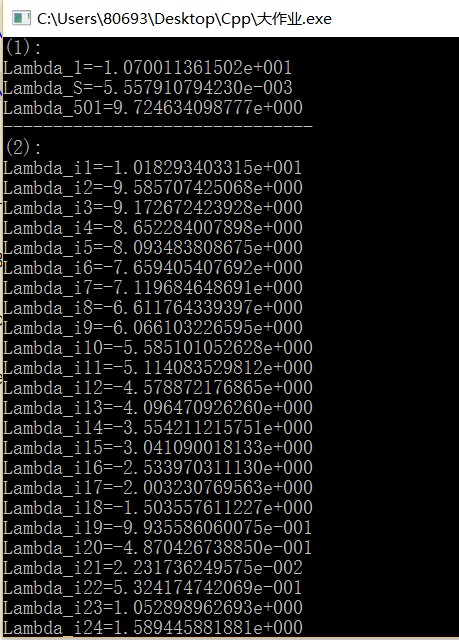
\includegraphics[width=9cm]{1.jpg}
\caption{Result1} \label{fig:1}
\end{figure}

\begin{figure}[h]
\small
\centering
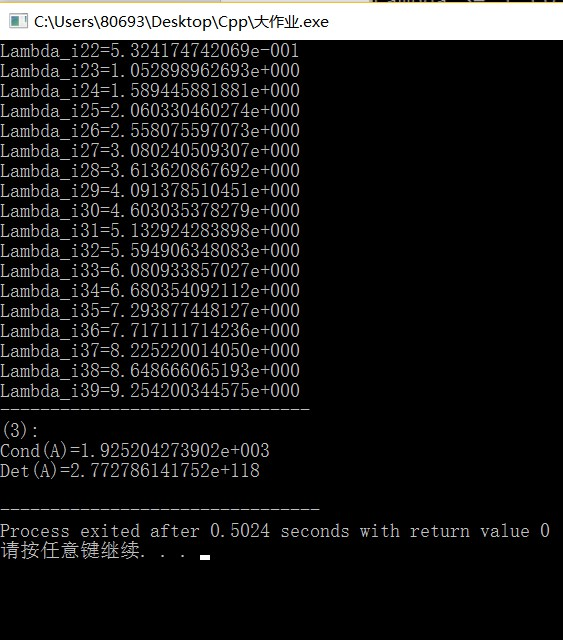
\includegraphics[width=12cm]{2.jpg}
\caption{Result2} \label{fig:2}
\end{figure}

\chapter{讨论}
当我第一次运行幂法的程序时,所使用的初始向量为u[1]=1,u[i]=0(i=2,3$\cdots$500),
所得到的结果为$\lambda_1=-2.080981085336e+000$,
而此时我已知正确答案是$\lambda_1=-1.070011361502e+001$。

反复检查程序后,并没有发现程序出现问题,
为了验证,我用MATLAB程序也写了一个幂法求特征值的程序,
然而跑出来的$\lambda_1$的值依旧为-2.08。
由于MATLAB程序简单明了,出现错误的几率很小。
于是我又写了个程序,随机生成$N\times N$的稀疏矩阵,
并将其程序的计算结果和Mathematica计算出的结果比较,
几乎全部吻合,这让我更困惑了。
于是我用Mathematica将所有的特征值都求了出来,
仔细分析,发现-2.08恰好也是该矩阵的特征值,
那么显然是算法出了问题,使得前面的特征值都被跳过了。

\begin{figure}[h]
\small
\centering
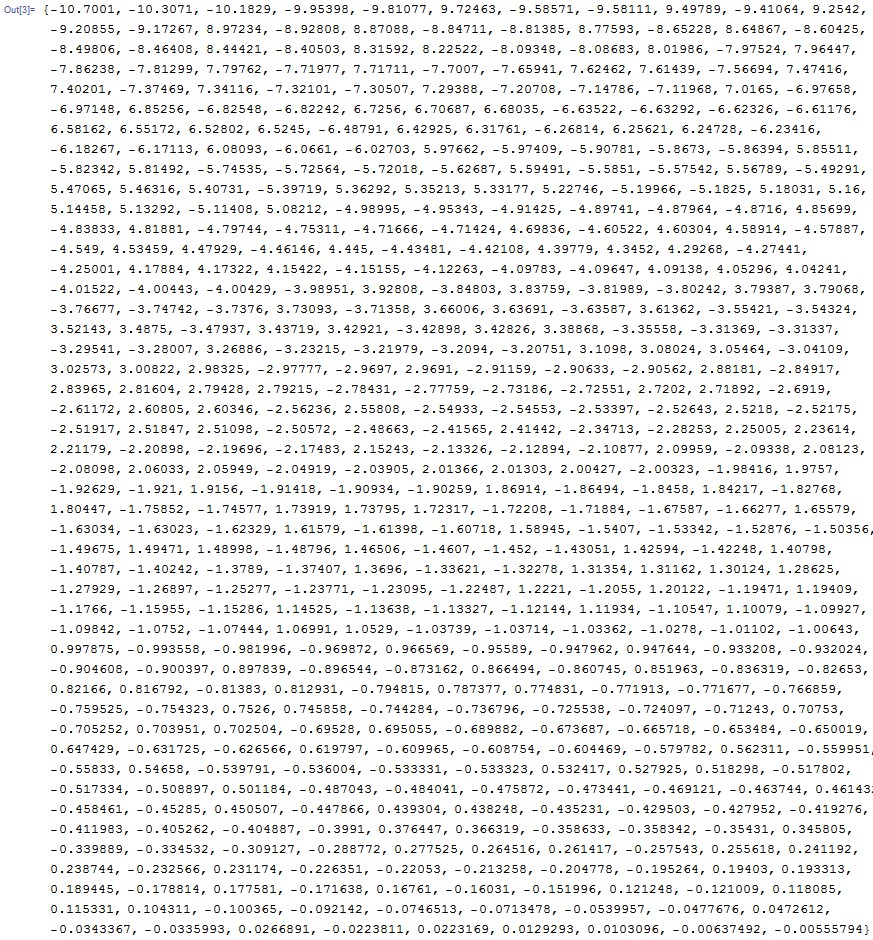
\includegraphics[width=17cm]{4.jpg}
\caption{Result of Eigenvalues} \label{fig:1}
\end{figure}
那么算法的问题出在哪里呢?
我们再仔细分析算法,观察以下两个式子
\[{u_0} = {\alpha _1}{x_1} + {\alpha _2}{x_2} + ... + {\alpha _n}{x_n}\]

\[{u_k} = \lambda _1^k\left[ {{\alpha _1}{x_1} + {\alpha _2}{{\left( {\frac{{{\lambda _2}}}{{{\lambda _1}}}} \right)}^k}{x_2} +  \cdots  + {\alpha _n}{{\left( {\frac{{{\lambda _n}}}{{{\lambda _1}}}} \right)}^k}{x_n}} \right]\]

向量$\bm{u}_0$被分解成特征向量$\bm{x}_k(k=1,2,\cdots,n)$的线性组合,
但当$\alpha_1=0,\alpha_\ne 0$时,
\[\mathop {\lim }\limits_{k \to \infty } {u_k} \approx \lambda _1^k{a_2}{{\bm{x}}_1}\]
那么,程序的问题应该是$\alpha_1=\alpha_2=\cdots=0$,
使得-2.08前的特征向量的$\alpha_k$的值都为0。

结论:虽然算法上说$\bm{u}_0$的值是可以任取的,但当初始向量$\bm{u}_0$中的0元素较多时,将使得比较多的$\alpha_i=0$,此时计算出的结果与真实值差距较大。







\end{document}